\fig{fv:o7:diffraction}{不同路径的相位在同一探测点比较，波长不等于粒子的轨迹}{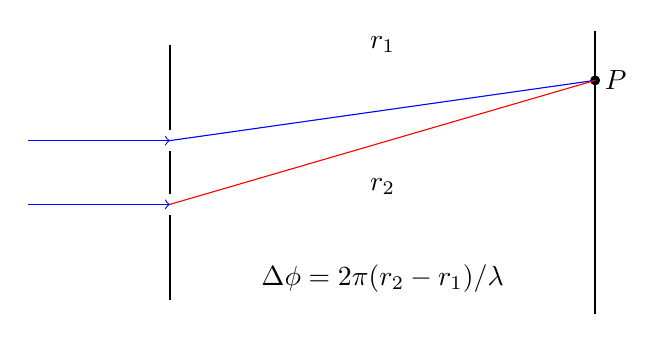
\begin{tikzpicture}[scale=.9]
\draw[thick](0,-1.8)--(0,-.6) (0,-.3)--(0,.3) (0,.6)--(0,1.8);
\draw[thick](6,-2)--(6,2);\fill(6,1.3)circle(2pt)node[right]{$P$};
\draw[->,blue](-2,.45)--(0,.45);\draw[->,blue](-2,-.45)--(0,-.45);
\draw[blue](0,.45)--(6,1.3);\draw[red](0,-.45)--(6,1.3);
\node at(3,1.8){$r_1$};\node at(3,-.2){$r_2$};\node at(3,-1.5){$\Delta\phi=2\pi(r_2-r_1)/\lambda$};
\end{tikzpicture}}
图\ref{fv:o7:diffraction}中的线段用来比较两条传播路径的相位，不能解释成电子同时沿两条确定的经典轨迹运动。动量确定空间相位的尺度 $\lambda=h/p$，到达 $P$的概率则由相应概率幅相加后取模平方得到。单个电子的探测是一个局域事件，多次重复才逐渐显示空间分布。若到达 $P$ 的两路概率幅分别为 $\psi_1(P),\psi_2(P)$，且没有区分路径的测量，则
\[
 \mathcal P(P)\propto|\psi_1+\psi_2|^2
 =|\psi_1|^2+|\psi_2|^2+2\operatorname{Re}(\psi_1^*\psi_2).
\]
图中的路程差进入最后一项的相位。被探测到的每个电子仍贡献一个局域记录；积累的空间分布检验的是这些记录的概率，不能把波长解释成单个电子在图中的上下摆动幅度。
